\documentclass[titlepage,11pt]{scrartcl}
\usepackage{graphicx}
\usepackage[utf8]{inputenc}
\usepackage{amsmath}
\usepackage{amsmath}
\usepackage{amsfonts}
\usepackage{amssymb}
\usepackage{listings}
\usepackage[pdftex]{hyperref}
\usepackage[x11names,table]{xcolor}
\usepackage{graphicx}
\usepackage{float}

\title{	
    \normalfont\normalsize
	\vspace{25pt}
	{\huge Simulación-Programación Declarativa\ Proyecto 2}
	\vspace{12pt}
}

\author{\LARGE Enrique Martínez González C-412}

\date{}

\begin{document}

\maketitle

\section{Orden del problema asignado:}
\subsection{Marco General:}
El ambiente en el cual intervienen los agentes es discreto y tiene la forma de un rectángulo de NxM. El ambiente es de información completa, por tanto todos los agentes conocen toda la información sobre el agente. El ambiente puede variar aleatoriamente cada t unidades de tiempo. El valor de t es conocido.

Las acciones que realizan los agentes ocurren por turnos. En un turno, los agentes realizan sus acciones, una sola por cada agente, y modifican el medio sin que este varíe a no ser que cambie por una acción de los agentes. En el siguiente, el ambiente puede variar. Si es el momento de cambio del ambiente, ocurre primero el cambio natural del ambiente y luego la variación aleatoria. En una unidad de tiempo ocurren el turno del agente y el turno de cambio del ambiente.

Los elementos que pueden existir en el ambiente son obstáculos, suciedad, niños, el corral y los agentes que son llamados Robots de Casa. A continuación se precisan las características de los elementos del ambiente:

\begin{itemize}
    \item Obstáculos: estos ocupan una única casilla en el ambiente. Ellos pueden ser movidos, empujándolos, por los niños, una única casilla. El Robot de Casa sin embargo no puede moverlo. No pueden ser movidos ninguna de las casillas ocupadas por cualquier otro elemento del ambiente.
    \item Suciedad: la suciedad es por cada casilla del ambiente. Solo puede aparecer en casillas que previamente estuvieron vacías. Esta, o aparece en el estado inicial o es creada por los niños.
    \item Corral: el corral ocupa casillas adyacentes en número igual al del total de niños presentes en el ambiente. El corral no puede moverse. En una casilla del corral solo puede coexistir un niño. En una casilla del corral, que esté vacía, puede entrar un robot. En una misma casilla del corral pueden coexistir un niño y un robot solo si el robot lo carga, o si acaba de dejar al niño.
    \item Niño: los niños ocupan solo una casilla. Ellos en el turno del ambiente se mueven, si es posible (si la casilla no está ocupada: no tiene suciedad, no está el corral, no hay un Robot de Casa), y aleatóriamente (puede que no ocurra movimiento), a una de las casilla adyacentes. Si esa casilla está ocupada por un obstáculo este es empujado por el niño, si en la dirección hay más de un obstáculo, entonces se desplazan todos. Si el obstáculo está en una posición donde no puede ser empujado y el niño lo intenta, entonces el obstáculo no se mueve y el niño ocupa la misma posición. Los niños son los responsables de que aparezca suciedad. Si en una cuadrícula de 3x3 hay un solo niño, entonces, luego de que él se mueva aleatoriamente, una de las casillas de la cuadrícula anterior que esté vacía puede haber sido ensuciada. Si hay dos niños se pueden ensuciar hasta 3. Si hay tres niños o más pueden resultar sucias hasta 6. Los niños cuando están en una casilla del corral, ni se mueven ni ensucian. Si un niño es capturado por un Robot de Casa tampoco se mueve ni ensucia.
    \item Robot de Casa: El Robot de Casa se encarga de limpiar y de controlar a los niños. El Robot se mueve a una de las casillas adyacentes, las que decida. Solo se mueve una casilla sino carga un niño. Si carga un niño puede moverse hasta dos casillas consecutivas. También puede realizar las acciones de limpiar y cargar niños. Si se mueve a una casilla con suciedad, en el próximo turno puede decidir limpiar o moverse. Si se mueve a una casilla donde está un niño, inmediatamente lo carga. En ese momento, coexisten en la casilla Robot y niño. Si se mueve a una casilla del corral que está vacía, y carga un niño, puede decidir si lo deja esta casilla o se sigue moviendo. El Robot puede dejar al niño que carga en cualquier casilla. En ese momento cesa el movimiento del Robot en el turno, y coexisten hasta el próximo turno, en la misma casilla, Robot y niño.2. Objetivos El objetivo del Robot de Casa es mantener la casa limpia. Se considera la casa limpia si el 60\% de las casillas vacías no están sucias.
\end{itemize}

\section{Principales ideas seguidas para la solución del problema:}
Para comenzar el simulado del problema planteado se crea una habitación representada por una cuadrícula de $N$ por $M$, en la que cada celda poseerá un tipo en el entorno de la habitación, estos tipos pueden ser varios y representan todos los posibles estados en los que se puede encontrar una casilla. Esta cuadrícula la llamaremos tablero y encima de este es donde ocurren todos los enventos. En un comienzo se generan encima de este la cantidad de niños, robots, corrales, obstáculos y basura que introduzca el usuario, además selecciona el tipo de modelo de agente que desea utilizar para la realización de la simulación, resaltar que las dimensiones del tablero son escogidas igualmente por el usuario.

Una vez que se posee un tablero inicial, comienza el simulado con las características mencionadas en la orientación. Primeramente se desplazan los niños si le corresponde en ese turno, pues el usuario introdujo la cantidad $T$ de turnos que tienen que suceder para que el ambiente cambie, este cambio de ambiente es el desplazamiento de los niños y la generación de basura si corresponde. Los niños se desplazan con probabilidad $1/2$ y una vez desplazados se genera basura con probabilidad $1/2$ en todas las cuadriculas de $3$ por $3$ en las que estaba presente justo antes de desplazarse siguiendo las normas de generación de basura planteadas en la orientación.

Con todos los niños en el lugar que le corresponde, se procede a mover los roboces presentes en el tablero, siguiendo el modelo seleccionado por el usuario. En la implementación existen 3 modelos de agentes, los tres se diferencian en la acción que realizan cuando se encuentra el robot solo en una casilla. Si el robot está sobre una casilla sucia, este la limpiará siempre, si está encima de una casilla con un niño, este lo cargara siempre, si está cargando un niño buscará el corral más cercano y si ya está encima de un corral, dejará al niño en este sitio, si ya lo había dejado pues tendrá el mismo comportamiento que si estuviese en una casilla vacía, que a su vez es el mismo comportamiento del robot cuando se encuentra en un corral vacío. Ahora, cuál es el comportamiento de un robot encima de una de estas casillas. Pues es en esta desición en la que varían los modelos implementados. En el primero de ellos, el robot irá tras el niño más cercano, en el segundo irá a limpiar la basura más cercana y en el tercero irá a por el niño o basura más cercana. En los dos primeros, en caso de que no exista su objetivo, buscará la basura más cercana en caso del primer modelo o el niño más próximo en caso del segundo. En caso que no exista basura o niño alcanzable solo mantendrá su posición. En el tercer modelo en caso de que no exista basura o niño alcanzable sencillamente no se moverá. Resaltar el caso que el robot cargue a un niño y no existan corrales alcanzables, el robot limpiará la basura más cercana.

La simulación culmina cuando se alcanza una cantidad de turnos máximas o cuando la habitación posee el 60\% de las casillas vacías limpias como indica la orientación del problema.

Para una mejor observación de la simulación se imprime en la consola el estado del tablero a lo largo de los turnos, las casillas son representadas por una matriz, en la que cada casilla puede poseer un máximo de 3 letras representando el tipo que está ocupando la celda en ese instante. A continuación se muestra el significado de cada posible estado de las celdas de esta cuadrícula:

\begin{itemize}
    \item vacío = "[\ \ \ ]"
    \item robot = "[ R ]"
    \item niño = "[ C ]"
    \item basura = "[ T ]"
    \item corral = "[ H ]"
    \item obstáculo = "[ X ]"
    \item robot y basura = "[RT ]"
    \item robot y niño = "[RC ]"
    \item robot y corral = "[RH ]"
    \item niño y corral = "[CH ]"
    \item robot, niño y corral = "[RCH]"
    \item robot, niño y basura = "[RCT]"
\end{itemize}

\section{Modelos de agentes considerados:}
Para la simulación planteada en la orientación se crearon 3 modelos de agentes que su principal diferencia es la acción que realiza el robot cuando se encuentra en una casilla vacía, en una casilla con un corral vacío o en una casilla con un corral y un niño pero este ya ha sido dejado en un turno anterior. Para el resto de estados se comporta de la siguiente forma:
\begin{itemize}
    \item robot solo encima de basura: limpia la basura.
    \item robot con niño encima de basura: limpia la basura.
    \item robot con niño encima de una casilla libre: se dirige hacia el corral vacío más cercano.
    \item robot encima de un corral con un niño sin haberlo colocado: coloca al niño en este corral.
\end{itemize}
Uno de los agentes solamente tiene preferencia por el niño o basura más cercana, este se podría considerar puramente reactivo, ya que cumple con la definición plasmada en el libro Temas de Simulación.
\begin{quotation}
    Ciertos tipos de agentes deciden que hacer sin hacer referencia a su historia. Ellos basan su decisión enteramente en el presente, sin referencia a todo lo pasado. A este tipo de agentes los llamaremos agentes puramente reactivos, debido a que simplemente responden directamente al ambiente.
\end{quotation}
En caso de los otros dos agentes, tienen una estrategia definida por la preferencia a un tipo de celda, en caso de el que posee preferencia por los niños, este buscará al niño más cercano para llevarlo al corral más próximo y así impedir que el niño siga generando suciedad y el otro prefiere eliminar toda la basura cercana intentando alcanzar la limpieza en la habitación ya que este es el objetivo de la simulación. Ambos se podría decir que son más proactivos que reactivos ya que muestran un comportamiento $goal-directed$, tomando la iniciativa de seguir el camino más cercano para lograr sus objetivos.


\section{Ideas seguidas para la implementación:}
Para la represetación del tablero se utilizó una lista de listas en la que cada casilla contiene sus coordenadas para una facilidad en su empleo, y el tipo de celda en cuestión, además de dos propiedades más que indican si se está dejando algo o recogiendo algo, estas existen para que puedan coexistir robots y niños en una misma casilla en múltiples estados.

El tablero inicial es en comienzo una cuadrícula de $N$ filas y $M$ columnas en el que todas las casilas son de tipo $empty$. Para la generación de los distintos tipos de celdas en el tablero inicial se utiliza una selección aleatoria de una cantidad igual a la escogida por el usuario del tipo de casilla en específico sobre una lista de todas las celdas de tipo $empty$ que se encuentran en el tablero en ese momento. El caso de corrales es especial pues estos deben estar adyacentes. Para esto se crea en comienzo un corral en una posición aleatoria, y luego se van generando corrales en una casilla adyacente vacía a un corral aleatorio de los ya colocados hasta llegar a la cantidad de corrales igual a la cantidad de niños seleccionadas en un comienzo.

Una vez creado el tablero se desplazan los niños. Estos se mueven cada $T$ turnos, con una probabilidad de $1/2$ cada niño, esta probabilidad es facilmente modificable en el código. Si en la dirección que este se va a mover existe un obstáculo, se busca la primera casilla libre en la dirección del movimiento a realizar para poder desplazar todos los obstáculos en esta dirección, en caso de que no exista, el niño mantiene su posición. En caso de que el movimiento del niño sea satisfactorio se procede a generar basura, esta se crea buscando todas las subcuadrículas de $3$ por $3$ a las que pertenecía el niño, por cada subcuadrícula se cuenta la cantidad de niños que hay dentro de las 9 celdas y la cantidad de basura que hay en estas. Dados estos números se sabe el número máximo de basura que se puede generar, en caso de que sea mayor que 0, se recorre cada celda de la subcuadrícula y se genera basura con probabilidad $1/2$, resaltar que esta probabilidad se puede modificar facilmente en la implementación, una vez se acaban las celdas en la subcuadrícula o se llega al máximo de basura permitido, se pasa a la siguiente subcuadrícula.

Con los niños desplazados, se mueven los roboces pertenecientes al tablero resultante. Con este fin cada estado de un robot tiene un objetivo en su movimiento. Este objetivo cambia con respecto al modelo seleccionado en un comienzo por el usuario para los estados en los que un robot está solo, está en un corral vacío o está en un corral con un niño pero ya lo dejó en un turno anterior. Para cumplir el objetivo correspondiente a cada estado en los tres modelos se realiza un búsqueda de la casilla que satisface la condición de ser la celda deseada más cercana, para esto se implementó una matriz de distancia que se expande desde el robot analizado en ese instante, en donde no puede atravesar los tipos de celdas que no pueden poseer un robot encima especificados en la orientación y se toma de los objetivos el que menor distancia con respecto al robot tenga. Con esta misma matriz de distancia se genera el camino que debe tomar el robot y así saber que dirección debe tomar este en el turno. Con la trayectoria que debe serguir el robot se realiza el movimiento para acercar a este a la celda deseada. En caso de que la celda deseada no exista, o no sea accesible, el robot busca otro objetivo secundario de menor importancia, en caso del modelo que prioriza la recogida de niños, su objetivo secundario es la basura, y en el modelo que su casilla deseada es la basura, al no poder llegar a esta, buscará a un niño, el modelo que busca el objeto más cercano no posee objetivo secundario. Si en la trayectoria un robot coincide con una basura, este la limpia, y si coincide con un niño este lo carga. Si un robot tiene un niño cargado, su objetivo principal en todos los modelos es dejarlo en un corral y su objetivo secundario es la basura. En caso de que un robot no pueda cumplir su objetivo primario ni secundario, este mantendrá su posición sin realizar ninguna acción.

La simulación correrá mientras la cantidad de turnos transcurridos sea menor que el máximo fijado, resaltar que esta cantidad máxima de turnos puede ser modificada facilmente en el código en el que por defecto está con un máximo de $1000$ turnos, y mientras la cantidad de casillas limpias sea menor al 60\% de las casillas ensuciables en el tablero.

\section{Consideraciones obtenidas a partir de la ejecución de las simulaciones del problema:}
Luego de varias simulaciones dados distintos paramétros se logra apreciar como con estos modelos planteados en la solución, uno limpia la habitación más rápido que el resto en dependencia fundamental de la cantidad de turnos que deben suceder para que los niños se muevan. En la gráfica \ref{fig:simulation} se puede apreciar la cantidad de turnos que demoran los distintos agentes para tener limpia la habitación modificando el valor de $T$. En este ejemplo se utilizó una habitación de $50$ filas y $50$ columnas, una cantidad de $500$ obstáculos, $100$ niños junto a $20$ roboces y una cantidad inicial de $1500$ basuras, todo esto con semilla $0$ El agente que tiene como objetivo principal la basura comienza a ser mejor, definiendo mejor como el agente que consigue limpiar la habitación más rápido, a partir de un valor de $T$ ya que al generarse menos basura a lo largo de la ejecución, no es fundamental recoger a niños e impedir que estos generen más casillas sucias.

\begin{figure}[htb]
    \begin{center}
        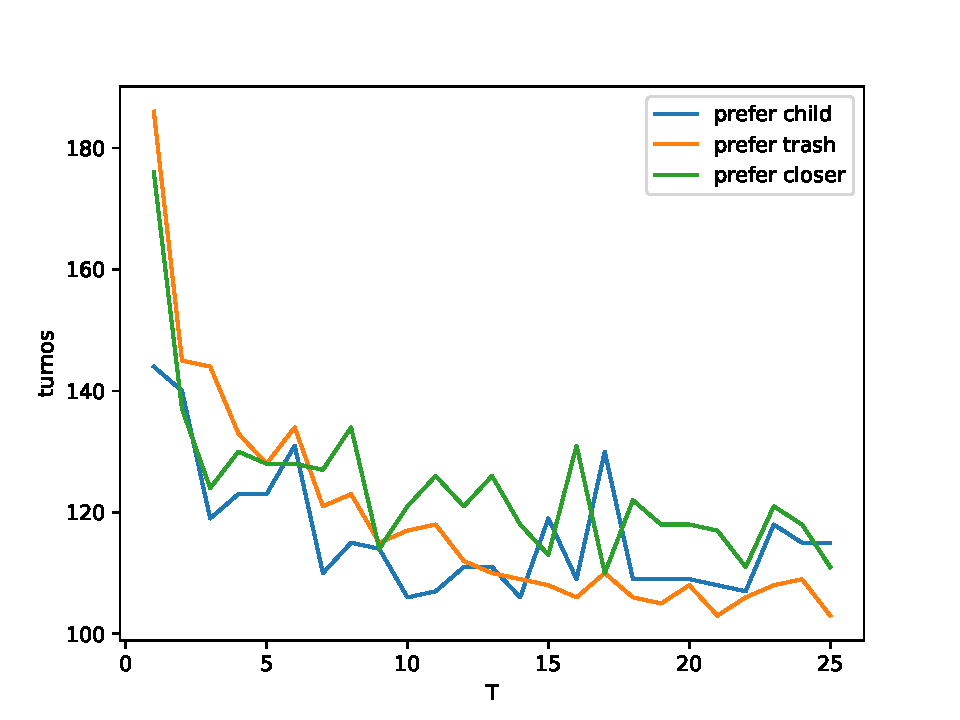
\includegraphics[width=\columnwidth]{./media/simulation.pdf}
    \end{center}
    \caption{Simulación de una habitación\label{fig:simulation}}
\end{figure}

El agente que sencillamente prefiere el más cercano posee un comportamiento un tanto aleatorio pero en general sigue siendo peor que el que prefiere recoger la basura.

\section{Enlace al repositorio del proyecto en Github:}
\url{https://github.com/kikeXD/simulation-haskell}
\end{document}